\documentclass[12pt]{article}

\usepackage[T1]{fontenc}
\usepackage{graphicx, amsfonts, palatino}
\usepackage{multicols, verse, color}

% Setting pagesize to widescreen format
\setlength{\paperwidth}{178mm}
\setlength{\paperheight}{100mm}
\setlength{\paperwidth}{0.75\paperwidth}
\setlength{\paperheight}{0.75\paperheight}
%\setlength{\paperwidth}{267mm}
%\setlength{\paperheight}{150mm}
\pdfpagewidth=\paperwidth
\pdfpageheight=\paperheight

%Setting margin
\setlength{\hoffset}{-1in}%2
\setlength{\oddsidemargin}{0pt}%3
\setlength{\marginparsep}{0pt}%9
\setlength{\marginparwidth}{0pt}%10

%Setting header
\setlength{\voffset}{-1in}%2
\setlength{\topmargin}{0pt}%4
\setlength{\headheight}{0pt}%5
\setlength{\headsep}{0pt}%6

%Setting fotter
\setlength{\footskip}{0pt}%11

%Setting hoffset and voffset
\addtolength{\hoffset}{5mm}
\addtolength{\voffset}{10mm}

%Setting textsize
\setlength{\textwidth}{\paperwidth}
\addtolength{\textwidth}{-10mm}
\setlength{\textheight}{\paperheight}
\addtolength{\textheight}{-20mm}

\newcommand{\alignment}[1]{
\rule{0.1pt}{0.1pt}\vspace{0.1cm}

#1
}

\newcommand{\attrib}[1]{%
  \nopagebreak{\raggedleft\footnotesize #1 \par}
}

\newcommand{\versestart}{
  \rule{0.1pt}{0.1pt}
  \vspace{\stretch{1}}
}

\newcommand{\verseend}{
  \vspace{\stretch{2}}
  \rule{0.1pt}{0.1pt}
  \newpage
}

\newcommand{\versetitle}[2]{
  \rule{0.1pt}{0.1pt}
  \vspace{\stretch{1}}

  \hspace{\stretch{1}}\textbf{\large{#1}}\hspace{\stretch{1}}
  \rule{0.1pt}{0.1pt}\\[-5pt]

  \hspace{\stretch{1}}melodi: #2\hspace{\stretch{1}}
  \vspace{\stretch{3}}
  \newpage
}



\newcommand{\pause}{\newpage%\pagecolor{black}
\rule{0.1pt}{0.1pt}\newpage %\pagecolor{black}
}


\parindent=0pt

\pagestyle{empty}

\begin{document}

\color{white}
\pagecolor{black}
\alignment{
  \begin{center}
  \begin{Huge}
  \textbf{\textsc{Velkommen til}}\\[10pt]
  \textbf{\textsc{Matematikrevy 2007}}
  \end{Huge}
  \end{center}
}

\pause

\versetitle{Introsang}{Backstreet Boys --- As long as you love me}

\settowidth{\versewidth}{Vi har brugt over en m�ned p� at �v' det her,}
\versestart
\begin{verse}[\versewidth]
Vi har brugt over en time p� at �v' det her,\\
S� pr�v nu for fa'en at f�lg' med.\\
I er vidne til en kvalitetsrevy,\\
Som vi fuldt og fast kan st� ved.\\
\end{verse}
\verseend

\versestart
\settowidth{\versewidth}{Vi ved godt, I har lagt en masse penge her,}
\begin{verse}[\versewidth]
Vi ved godt, I har lagt en masse penge her,\\
Dem bruger vi nok p� lidt snaps.\\
Men selv om I er bankelamme ud'n man�r',\\
S� m� der gerne klap's...
\end{verse}
\verseend

\versestart
\settowidth{\versewidth}{Vi ved godt, hvem I er}
\begin{verse}[\versewidth]
Vi ved godt, hvem I er\\
Hvor I bor\\
I er safe\\
S� l�nge I klapper.\\
\end{verse}
\verseend

\versestart
\settowidth{\versewidth}{Vi ved godt, hvem I er}
\begin{verse}[\versewidth]
Hvem I er\\
Hvor I bor\\
Men I kommer hjem\\
S� l�nge I klapper.\\
S� l�nge I klapper.
\end{verse}
\verseend

\versestart
\settowidth{\versewidth}{For vi lever af jer's k�rlighe}
\begin{verse}[\versewidth]
Uden jer er salen hul og tom\\
Det var godt I kom\\
S� vi ikke er alene\\
For vi lever af jer's k�rlighed\\
S� l�nge I klapper, yeah yeah
\end{verse}
\verseend

\versestart
\settowidth{\versewidth}{Vi ved godt, hvem I er}
\begin{verse}[\versewidth]
Vi ved godt, hvem I er\\
Hvor I bor\\
I er safe\\
S� l�nge I klapper.\\
\end{verse}
\verseend

\versestart
\settowidth{\versewidth}{Vi ved godt, hvem I er}
\begin{verse}[\versewidth]
Hvem I er\\
Hvor I bor\\
Men I kommer hjem\\
S� l�nge I klapper.\\
S� l�nge I klapper.
\end{verse}
\verseend

\pause

\alignment{
  \begin{center}
  \begin{Large}
  \textbf{Nummer 1}\\[10pt]
  Det er en d�dssynd at bruge �ben ild
  \end{Large}
  \end{center}
}\newpage

\alignment{
  \begin{center}
  \begin{Large}
  \textbf{Nummer 2}\\[10pt]
  Mobiltelefoner har Fanden skabt\\[5pt]
  \end{Large}
  Det er derfor, under vores hellige revy, ikke tilladt at have disse t�ndt
  \end{center}
}\newpage

\alignment{
  \begin{center}
  \begin{Large}
  \textbf{Nummer 3}\\[10pt]
  Det er helligebr�de at spilde jeres s�d ud over vores revy, s�vel som over den golde jord.
  \end{Large}
  \end{center}
}\newpage

\alignment{
  \begin{center}
  \begin{Large}
  \textbf{Nummer 4}\\[10pt]
  Festen foreg�r efter revyen i Vandrehallen\\[5pt]
  \end{Large}
  Husk at rygning er tabu
  \end{center}
}\newpage

\alignment{
  \begin{center}
  \begin{Large}
  \textbf{Nummer 5}\\[10pt]
  Jorden udg�r Universets centrum\\[5pt]
  \end{Large}
  Det er et faktum, og hvis nogen af jer skulle n�gte det, kan vi midlertidigt oph�ve bud nummer
  1 til en hurtig k�tterafbr�nding
  \end{center}
}

\pause

\alignment{
  \begin{center}
  \begin{Large}
  \textbf{Nummer 6}\\[10pt]
  Kiksekastere -- Vi holder �je med dig\\[5pt]
  \end{Large}
  Syndernes sj�l vil til evig tid blive forfulgt af special-kardinaler
  \end{center}
}\newpage

\alignment{
  \begin{center}
  \begin{Large}
  \textbf{Nummer 7}\\[10pt]
  Brug af pr�servativer kan ikke tolereres\\[5pt]
  \end{Large}
  Sex der ikke medf�rer befrugtigelse er uhelligt
  \end{center}
}\newpage

\alignment{
  \begin{center}
  \begin{Large}
  \textbf{Nummer 8}\\[10pt]
  Skulle dommedag eller lignende indtr�ffe,\\[5pt]
  \end{Large}
  kan du bruge en af n�dudgangene
  \end{center}
}\newpage

\alignment{
  \begin{center}
  \begin{Large}
  \textbf{Nummer 9}\\[10pt]
  Sodomi er tabubelagt\\[5pt]
  \end{Large}
  Dette inkludere dyre-, anal- og oralsex.
  \end{center}
}\newpage

\alignment{
  \begin{center}
  \begin{Large}
  \textbf{Nummer 10}\\[10pt]
  Revyen best�r af to akter\\[5pt]
  \end{Large}
  I pausen kan du forsyne dig med diverse drikkevarer
  \end{center}
}


\pause

\versetitle{Velkomst}{Side by side}

\versestart
\settowidth{\versewidth}{V�r velkommen her til revyen}
% \regi{mel: Side by side}
\begin{verse}[\versewidth]
V�r velkommen her til revyen\\
Den bedste af slagsen i byen\\
For vi laver straks\\
Sjov med al slags\\
Mat' ma tik
\end{verse}
\verseend

\versestart
\settowidth{\versewidth}{Vi ka skriv' s� sp�nd'ne beviser}
% \regi{mel: Side by side}
\begin{verse}[\versewidth]
Vi ka skriv' s� sp�nd'ne beviser\\
De ku vinde Pulitzer priser\\
Vi har halvn�gne pi'r\\
Der danser og si'r:\\
Mat' ma tik
\end{verse}
\verseend

\versestart
\settowidth{\versewidth}{Det bli'r sjover' n�r du' fulder'}
\begin{verse}[\versewidth]
Over scenen ruller\\
Sketches, sk�g og ballad'\\
Det bli'r sjover' n�r du' fulder'\\
S� drik dig syndig og glad!
\end{verse}
\verseend

\versestart
\settowidth{\versewidth}{Ja, h�v glasset h�jt og find gejsten}
\begin{verse}[\versewidth]
Ja, h�v glasset h�jt og find gejsten\\
Fyr den af med tryk 16\\
Indtil flasken er tom\\
Synger vi om\\
\textsc{mat' ma tik!}
\end{verse}
\verseend


\pause

\versetitle{Sangen om dataloger}{Hair --- ``Gi' mig hvide drenge''}

\versestart
\settowidth{\versewidth}{Langt og fedtet h�r}
\begin{verse}[\versewidth]
Giv mig dataloger\\
Store fede l�r\\
Giv mig dataloger\\
Langt og fedtet h�r
\end{verse}
\verseend

\versestart
\settowidth{\versewidth}{Eller spilder jeg min tid?!}
\begin{verse}[\versewidth]
Perler og rubiner\\
Si'r mig ikk' en skid\\
Kan du perl og ruby?\\
Eller spilder jeg min tid?!
\end{verse}
\verseend

\versestart
\settowidth{\versewidth}{Nogen siger at jeg er desperat}
\begin{verse}[\versewidth]
Dreng'ne ud' p� KUA\\
Dem dropper jeg fra nu af\\
Nogen siger at jeg er desperat\\
Det er da dem, der' for sart
\end{verse}
\verseend

\versestart
\settowidth{\versewidth}{Ser herrel�kker ud}
\begin{verse}[\versewidth]
Dataloger kilder\\
Gi'r mig g�sehud\\
Deres kildekode\\
Ser herrel�kker ud
\end{verse}
\verseend

\versestart
\settowidth{\versewidth}{Tror jeg br�nder sammen!}
\begin{verse}[\versewidth]
Store dataloger\\
Det er bar' s� fedt\\
Tror jeg br�nder sammen!\\
Det her er for hedt
\end{verse}
\verseend

\versestart
\settowidth{\versewidth}{Smukke kvinders software}
\begin{verse}[\versewidth]
Smukke kvinders software\\
kr�ver sikkerhed\\
Datalogens python -\\
Den g�r aldrig ned
\end{verse}
\verseend

\versestart
\settowidth{\versewidth}{Jeg syn's da jeg er for smart!}
\begin{verse}[\versewidth]
De andre humanister\\
Har ikke disse gnister\\
Venner siger je'er desperat\\
Jeg syn's da jeg er for smart!
\end{verse}
\verseend

\versestart
\settowidth{\versewidth}{Der' ik' noget der hedder}
\begin{verse}[\versewidth]
De vil gerne dele\\
Jeg er open source\\
Der' ik' noget der hedder\\
Mit og dit, kun vor's
\end{verse}
\verseend


\pause

\versetitle{Sangen om humanister}{Hair --- ``Gi' mig sorte drenge''}

\versestart
\settowidth{\versewidth}{Folk med Freud som gud!}
\begin{verse}[\versewidth]
Gi mig humanister\\
M�nd med charmeklud\\
Labre leninister,\\
Halvn�gne nudister,\\
Sorte satanister,\\
Folk med Freud som gud!
\end{verse}
\verseend

\versestart
\settowidth{\versewidth}{Sp�rg mig ikke hvoffer(, men)}
\begin{verse}[\versewidth]
Flotte filosoffer\\
Er han ikke smuk?\\
Det' det nemme offer,\\
Sp�rg mig ikke hvoffer(, men)\\
De har det med stoffer, som\\
Vi har det med druk!
\end{verse}
\verseend

\versestart
\settowidth{\versewidth}{Men hans "�jn'" er store!}
\begin{verse}[\versewidth]
S�de sociologer,\\
Der vil studere mig\\
Han bor hos sin moar,\\
Men hans "�jn'" er store!\\
Skal jeg end'lig score,\\
S� skal jeg ha' fransk!
\end{verse}
\verseend

\versestart
\settowidth{\versewidth}{Gi' mig humanister!}
\begin{verse}[\versewidth]
Humanister!\\
Gi' mig humanister!\\
\end{verse}
\verseend


\pause

\versetitle{Jeg er fysiker}{Monty Python --- Lumberjack}

\versestart
\settowidth{\versewidth}{Han kan sin Schaums bog uden ad!}
\begin{verse}[\versewidth]
Jeg er fysiker og jeg er glad\\
Jeg kan min Schaums bog uden ad!

Han er fysiker og han er glad\\
Han kan sin Schaums bog uden ad!
\end{verse}
\verseend

\versestart
\settowidth{\versewidth}{Jeg plotter i den farve,}
\begin{verse}[\versewidth]
Ampere her,\\
Promille der,\\
Jeg g�r et Maple-plot\\
Jeg plotter i den farve,\\
Min kone si'r er flot!
\end{verse}
\verseend

\versestart
\settowidth{\versewidth}{Han plotter i den farve,}
\begin{verse}[\versewidth]
Ampere her,\\
Promille der,\\
Han g�r et Maple-plot\\
Han plotter i den farve,\\
Hans kone si'r er flot!
\end{verse}
\verseend

\versestart
\settowidth{\versewidth}{Han kan sin Schaums bog uden ad!}
\begin{verse}[\versewidth]
Han er fysiker og han er glad\\
Han kan sin Schaums bog uden ad!
\end{verse}
\verseend

\versestart
\settowidth{\versewidth}{og leger med min rubikskube}
\begin{verse}[\versewidth]
Eksperimenter,\\
Analyser,\\
Og spis en masse slik!\\
Jeg l�ser en artikel,\\
og leger med min rubikskube
\end{verse}
\verseend

\versestart
\settowidth{\versewidth}{og leger med sin rubikskube\ldots}
\begin{verse}[\versewidth]
Eksperimenter,\\
Analyser,\\
Og spis en masse slik!\\
Han l�ser en artikel,\\
og leger med sin rubikskube\ldots
\end{verse}
\verseend

\versestart
\settowidth{\versewidth}{Jeg er fysiker, og jeg er fin,}
\begin{verse}[\versewidth]
Jeg er fysiker, og jeg er fin,\\
Jeg kan formlen for min urin!\\
\end{verse}
\verseend

\versestart
\settowidth{\versewidth}{Hvis blot jeg laved matmatik}
\begin{verse}[\versewidth]
Jeg r�kkeudvikler p� alt\\
Fordi det har jeg l�rt\\
Hvis blot jeg laved matmatik\\
som ham der Erik Kj�r!
\end{verse}
\verseend

\versestart
\settowidth{\versewidth}{Fordi det har han l�rt\ldots}
\begin{verse}[\versewidth]
Han r�kkeudvikler p� alt\\
Fordi det har han l�rt\ldots
\end{verse}
\verseend



\pause

%\addtolength{\paperwidth}{150mm}
\addtolength{\textwidth}{20mm}
\addtolength{\textheight}{50mm}
\addtolength{\hoffset}{-12mm}
\addtolength{\voffset}{-10mm}
\newpage
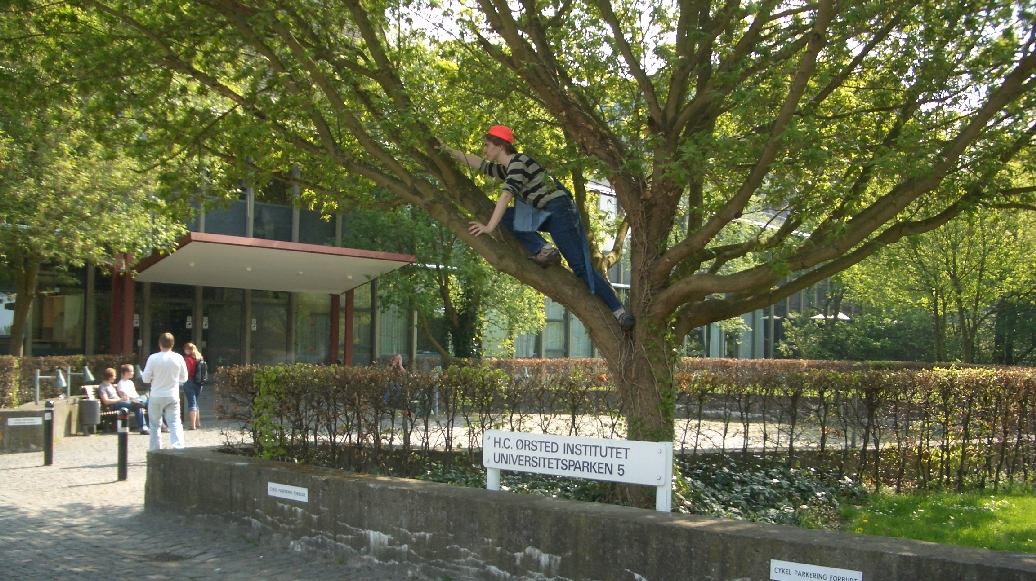
\includegraphics[width=\textwidth]{hco.jpg}
\newpage
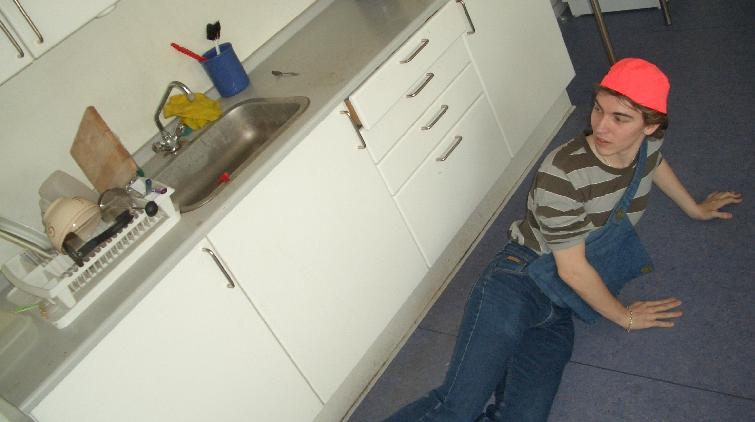
\includegraphics[width=\textwidth]{opvask.jpg}
\newpage
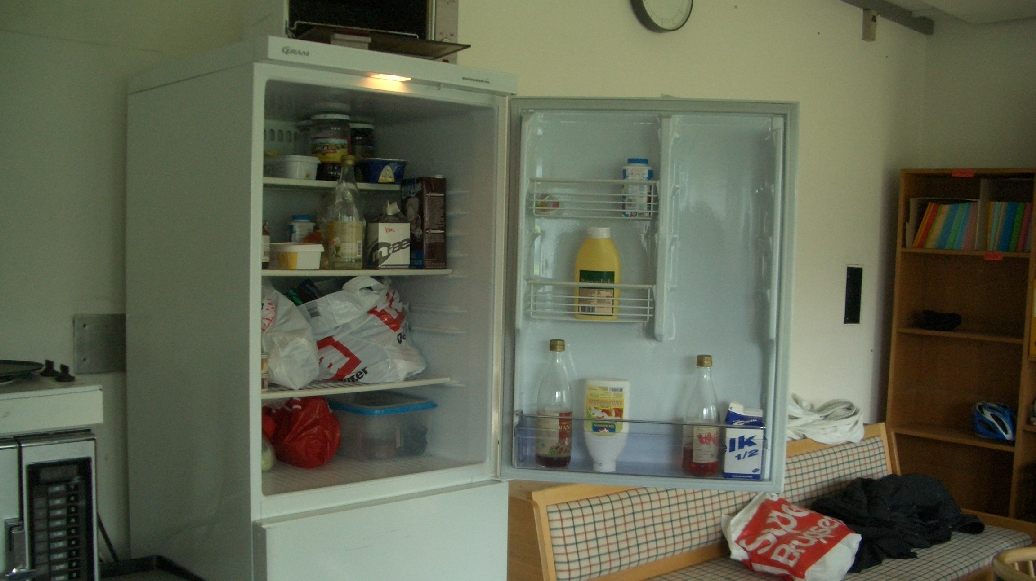
\includegraphics[width=\textwidth]{koleskab.jpg}
\newpage
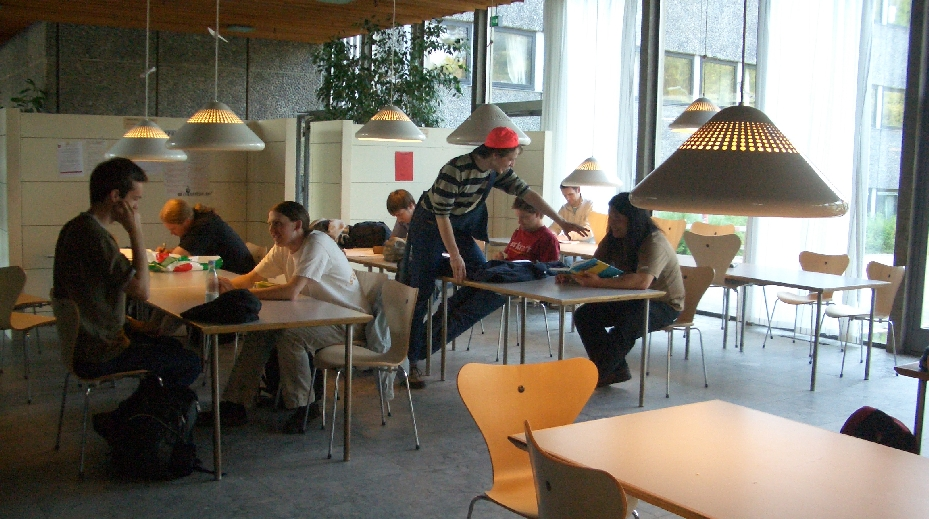
\includegraphics[width=\textwidth]{matKantinen.jpg}
\newpage
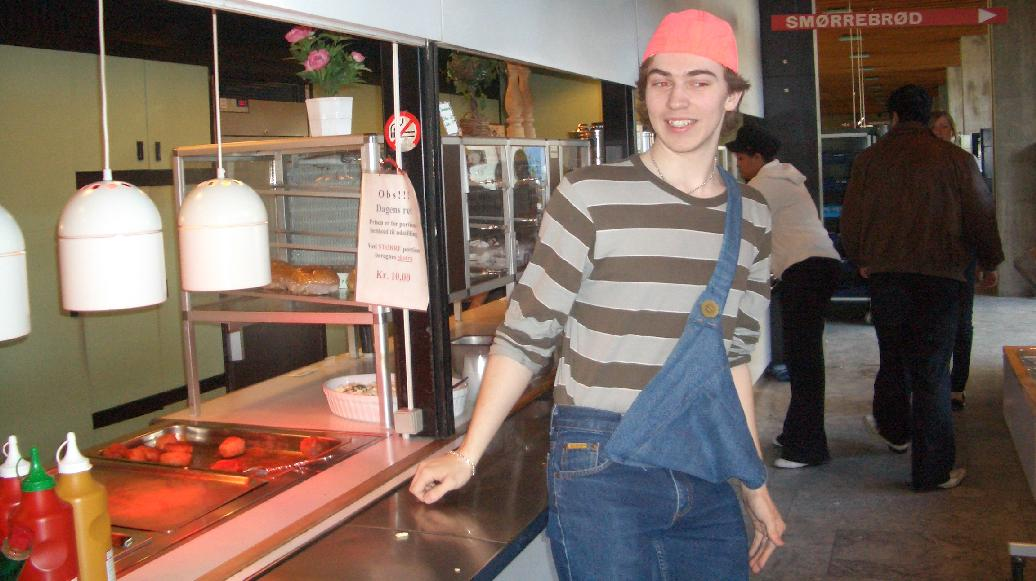
\includegraphics[width=\textwidth]{kantinen.jpg}
\newpage
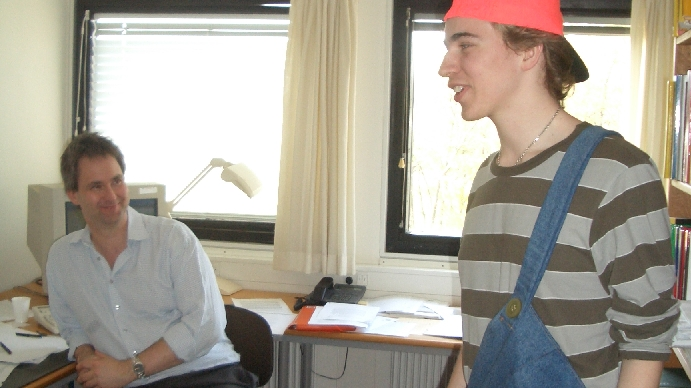
\includegraphics[width=\textwidth]{kontor.jpg}
\newpage
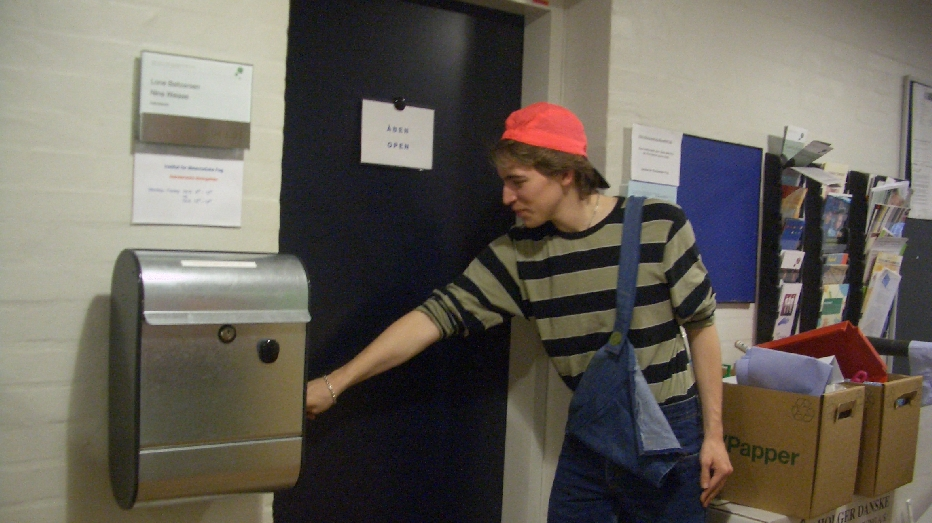
\includegraphics[width=\textwidth]{sekretariat.jpg}
\newpage
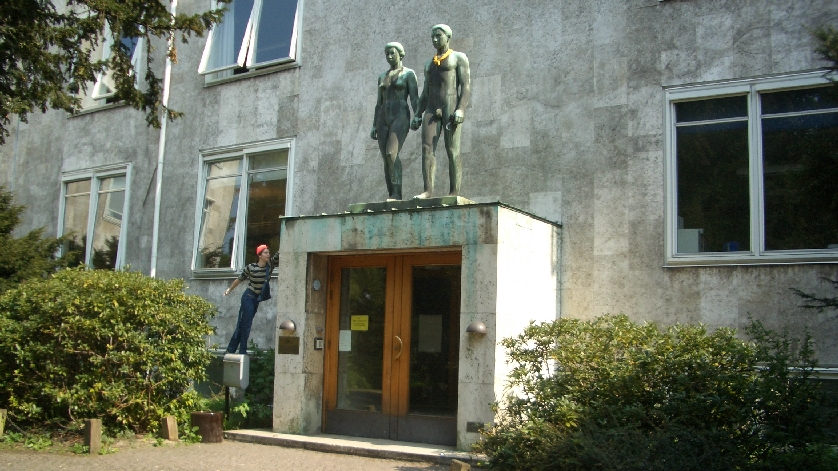
\includegraphics[width=\textwidth]{diku.jpg}
\newpage
\addtolength{\textwidth}{-20mm}
\addtolength{\textheight}{-50mm}
\addtolength{\hoffset}{12mm}
\addtolength{\voffset}{10mm}
\newpage

\pause

\versetitle{Fagfascist}{Natasja --- Op med hovedet}

\versestart
\settowidth{\versewidth}{Mat'matik aka sandheden - kom nu!}
\begin{verse}[\versewidth]
Euler er min helt\\
Cantor er min helt\\
Andre ka' g� hjem\\
Mat'matik aka sandheden - kom nu!
\end{verse}
\verseend

\versestart
\settowidth{\versewidth}{Mig humanist? Det ka' du godt ta' og glem!}
\begin{verse}[\versewidth]
Euler er min helt\\
Cantor er min helt\\
Andre ka' g� hjem\\
Mig humanist? Det ka' du godt ta' og glem!
\end{verse}
\verseend

\versestart
\settowidth{\versewidth}{Ku' jeg t�nk' mig en date en med teolog?}
\begin{verse}[\versewidth]
Ku  jeg t�nk' mig en date en med teolog?\\
Nix! For mig er det ikke nok at tro\\
Jeg vil vide noget om rummet $\mathbb{R}P^2$\\
Min elsker ska' v�re topolog
\end{verse}
\verseend

\versestart
\settowidth{\versewidth}{Jeg vil ha' fyr der tale algebra - yo\\}
\begin{verse}[\versewidth]
Om en musiker han kan spille ban-jo\\
Jeg vil ha' fyr der taler algebra - yo\\
P�dagog, sociolog og psykolog\\
Ingen af dem ved alt det om $\mathbb{Z}/2$\\
Yo yo yo
\end{verse}
\verseend

\versestart
\settowidth{\versewidth}{Et fag er et fag - mat'matik er min ven}
\begin{verse}[\versewidth]
Euler er min helt\\
Cantor er min helt\\
Andre ka' g� hjem\\
Et fag er et fag - mat'matik er min ven
\end{verse}
\verseend

\versestart
\settowidth{\versewidth}{Mig humanist? Det ka' du godt ta' og glem!}
\begin{verse}[\versewidth]
Euler er min helt\\
Cantor er min helt\\
Andre ka' g� hjem\\
Mig humanist? Det ka' du godt ta' og glem!
\end{verse}
\verseend

\versestart
\settowidth{\versewidth}{Ka' en jurist l�re mig den nyeste bedste geometri?}
\begin{verse}[\versewidth]
Ka' en jurist l�re mig den nyeste bedste geometri?\\
Jeg vil ikke elske med en fyr fra geologi\\
Kun med matematikken er jeg fri\\
Popsanger? - nix! - idolet er Cauchy
\end{verse}
\verseend

\versestart
\settowidth{\versewidth}{Hva' ska' jeg med en cand.mag i kunst?}
\begin{verse}[\versewidth]
Hva' ska' jeg med en cand.mag i kunst?\\
Jeg vil ha' en analytiker i brunst\\
l'Hopital - integral - diff'rential\\
Danse natten lang i Hilberts balsal
\end{verse}
\verseend

\versestart
\settowidth{\versewidth}{Et fag er et fag - mat'matik er min ven}
\begin{verse}[\versewidth]
Euler er min helt\\
Cantor er min helt\\
Andre ka' g� hjem\\
Et fag er et fag - mat'matik er min ven
\end{verse}
\verseend

\versestart
\settowidth{\versewidth}{Mig humanist? Det ka' du godt ta' og glem!}
\begin{verse}[\versewidth]
Euler er min helt\\
Cantor er min helt\\
Andre ka' g� hjem\\
Mig humanist? Det ka' du godt ta' og glem!
\end{verse}
\verseend

\versestart
\settowidth{\versewidth}{Syn's det lyder li's� slemt som fysik}
\begin{verse}[\versewidth]
Ka' jeg n�jes med en dreng fra musik?\\
Syn's det lyder li's� slemt som fysik\\
Ustringent og de fatter ik' en brik\\
Jeg har kun blik for logik
\end{verse}
\verseend

\versestart
\settowidth{\versewidth}{For hvis du begriber hvad Fermat han skriver}
\begin{verse}[\versewidth]
Holomorfi, isometri, m�lteori, homomorfi,\\
isomorfi, trigonometri\\
Kun matematik - det ka' jeg li'\\
Kommutativ, distributiv, associativ\\
\end{verse}
\verseend

\versestart
\settowidth{\versewidth}{For hvis du begriver hvad Fermat han skriver}
\begin{verse}[\versewidth]
For det' er mit liv!\\
Mat'matik er perfekt\\
Det andet er defekt\\
For hvis du begriber hvad Fermat han skriver\\
\end{verse}
\verseend

\versestart
\settowidth{\versewidth}{Mat'matik aka sandheden - kom nu!}
\begin{verse}[\versewidth]
Euler er min helt\\
Cantor er min helt\\
Andre ka' g� hjem\\
Mat'matik aka sandheden - kom nu!
\end{verse}
\verseend

\versestart
\settowidth{\versewidth}{Mig humanist? Det ka' du godt ta' og glem!}
\begin{verse}[\versewidth]
Euler er min helt\\
Cantor er min helt\\
Andre ka' g� hjem\\
Mig humanist? Det ka' du godt ta' og glem!
\end{verse}
\verseend



\pause

\versetitle{Sangen om bryster}{Monty Python --- The Money Song}

\versestart
\settowidth{\versewidth}{Hun har bryster der er p�nere end Bjarnes}
\begin{verse}[\versewidth]
\indentpattern{00110}
\begin{patverse}
Hun har bryster der er p�nere end Bjarnes. \\
Hun har bryster der kan f� os til at glo.\\
Hun har bryster, fler' end vi ku'\\
tro at vi sku' se p� DIKU.\\
Hun har bryster, ja rent faktisk har hun to.
\end{patverse}
\end{verse}
\verseend

\versestart
\settowidth{\versewidth}{Der er ingenting s� undersk�nt som bryster.}
\begin{verse}[\versewidth]
\indentpattern{00110}
\begin{patverse}
Der er ingenting s� undersk�nt som bryster.\\
Har man bryster kan man t�ve Djenghis Khan.\\
Bryster flytter bjerge, \\
mellem bryster bor der dv�rge.\\
Det var bryster der forpurred' Saurons plan.
\end{patverse}
\end{verse}
\verseend

\versestart
\settowidth{\versewidth}{og med bryster holder mister Spock sig varm.}
\begin{verse}[\versewidth]
\indentpattern{00110}
\begin{patverse}
Der er ingenting s� undersk�nt som bryster.\\
Der er intenting s� herligt som en barm.\\
Selv Darth Vader ryster, \\
n�r han h�rer ordet ``bryster'',\\
og med  bryster holder mister Spock sig varm.
\end{patverse}
\end{verse}
\verseend

\versestart
\settowidth{\versewidth}{kun med bryster, bryster, bryster kan man lykken n�!}
\begin{verse}[\versewidth]
Havde Luke haft bryster p�,
ville kejseren forst�:\\
kun med bryster, bryster, bryster kan man lykken n�!
\end{verse}
\verseend


\pause

\versetitle{Sangen om pik}{Monty Python --- The Money Song}

\versestart
\settowidth{\versewidth}{Han har fallos, der er flottere end neger'ns}
\begin{verse}[\versewidth]
\indentpattern{00110}
\begin{patverse}
Han har fallos, der er flottere end neger'ns\\
Han har penis, der kan f� os ned p� kn�\\
Og han fylder os med kriller\\
N�r han viser os sin diller\\
Har man penis kan man ordne et rel�
\end{patverse}
\end{verse}
\verseend

\versestart
\settowidth{\versewidth}{For hans tissemand st�r vores ben p� klem}
\begin{verse}[\versewidth]
\indentpattern{00110}
\begin{patverse}
Der er ingenting s� undersk�nt som pikke\\
Der er ingenting s� herligt som et lem\\
Vores �gtef�ller lider\\ 
N�r vi p� hans penis rider\\
For hans tissemand st�r vores ben p� klem
\end{patverse}
\end{verse}
\verseend

\versestart
\settowidth{\versewidth}{Der er ingenting s� undersk�nt som pikke}
\begin{verse}[\versewidth]
\indentpattern{00110}
\begin{patverse}
Der er ingenting s� undersk�nt som pikke\\
Med hans pik, s� kan man f� et leder-job\\
Selv den bedste pig' m� vige\\
N�r en pik skal til at stige\\
For med penis kan man komme helt til top
\end{patverse}
\end{verse}
\verseend

\versestart
\begin{verse}[\versewidth]
\settowidth{\versewidth}{Havde vi haft pikke p�, ville verden snart forst�}
Havde vi haft pikke p�, ville verden snart forst�\\
Kun med pikke, pikke, pikke kan man lykken n�!
\end{verse}
\verseend


\rule{0.1pt}{0.1pt}\vspace{5cm}

\rule{0.1pt}{0.1pt}
\vspace{\stretch{1}}
 
\hspace{\stretch{1}}\textbf{\Huge{\textsc{pause}}}\hspace{\stretch{1}}
 
\vspace{\stretch{2}}

\pause

\versetitle{V�gner p� sofa'n}{Dodo \& the Dodos --- V�gner i natten}

\versestart
\settowidth{\versewidth}{Dr�mmer lidt om GT og stomi.}
\begin{verse}[\versewidth]
Ligger jeg alene her?\\
Det h�ber jeg, jeg g�r.\\
Dr�mmer lidt om GT og stomi.
\end{verse}
\verseend

\versestart
\settowidth{\versewidth}{Men s� kom Caf�en?, og det blev alt for v�dt.}
\begin{verse}[\versewidth]
Det startede jo meget godt,\\
Til fredagss�sterfest.\\
Men s� kom Caf�en?, og det blev alt for v�dt.
\end{verse}
\verseend

\versestart
\settowidth{\versewidth}{M�rked' at det banked', banked' i mit bat.}
\begin{verse}[\versewidth]
Hun stod i baren og fik shots,\\
Vi drak den hele nat\\
M�rked' at det banked', banked' i mit bat.\\
Mon hun skal en tur p� sooofa-a-en?
\end{verse}
\verseend

\versestart
\settowidth{\versewidth}{Og omkring mig lugter der}
\begin{verse}[\versewidth]
V�gner p� sofa'n\\
I E-S01,\\
Og omkring mig lugter der\\
Lidt af toilet.\\
\end{verse}
\verseend

\versestart
\settowidth{\versewidth}{For jeg har kastet op p� gulvet,}
\begin{verse}[\versewidth]
For jeg har kastet op p� gulvet,\\
Tisset i en vask.\\
Uuh jeg kunne g�re det\\
Om igen og om og om igen.
\end{verse}
\verseend

\versestart
\settowidth{\versewidth}{Hun var stor og bumset: datalog!}
\begin{verse}[\versewidth]
(Hun) gav mig al sin k�rlighed,\\
Jeg gav et v�deskud.\\
Hun var stor og bumset: datalog!
\end{verse}
\verseend

\versestart
\settowidth{\versewidth}{Havd' jeg v�ret v�gen, da hun sad ov'n p� mig}
\begin{verse}[\versewidth]
Hun bar mig ned i S01\\
Og udnyttede mig.\\
Havd' jeg v�ret v�gen, da hun sad ov'n p� mig\\
Var jeg l�bet bort i cho-oook!
\end{verse}
\verseend

\versestart
\settowidth{\versewidth}{Og omkring mig lugter der}
\begin{verse}[\versewidth]
V�gner p� sofa'n\\
I E-S01,\\
Og omkring mig lugter der\\
Lidt af toilet.\\
\end{verse}
\verseend

\versestart
\settowidth{\versewidth}{For jeg har kastet op p� gulvet,}
\begin{verse}[\versewidth]
For jeg har kastet op p� gulvet,\\
Tisset i en vask.\\
Uuh jeg kunne g�re det\\
Om igen og om og om igen.
\end{verse}
\verseend

\versestart
\settowidth{\versewidth}{(Jeg) blev brutalt udnyttet af en kran\\}
\begin{verse}[\versewidth]
Nu hvor det hele lidt g�r op\\
For mig,\\
(Jeg) blev brutalt udnyttet af en kran\\
Fra DIIIII-KUUUUUU.
\end{verse}
\verseend

\versestart
\settowidth{\versewidth}{F�r jeg sure opst�d og kl�e i mit skridt.}
\begin{verse}[\versewidth]
N�r jeg ser tilbage p�\\
Den nat i S01,\\
F�r jeg sure opst�d og kl�e i mit skridt.\\
Jeg bli'r aldrig ren igeeeeeen!
\end{verse}
\verseend

\versestart
\settowidth{\versewidth}{Og omkring mig lugter der\\}
\begin{verse}[\versewidth]
V�gner p� sofa'n\\
I E-S01,\\
Og omkring mig lugter der\\
Lidt af toilet.\\
\end{verse}
\verseend

\versestart
\settowidth{\versewidth}{For jeg har kastet op p� gulvet,}
\begin{verse}[\versewidth]
For jeg har kastet op p� gulvet,\\
Tisset i en vask.\\
Uuh jeg kunne g�re det\\
Om igen og om og om igen.
\end{verse}
\verseend

\versestart
\settowidth{\versewidth}{Og omkring mig lugter der}
\begin{verse}[\versewidth]
V�gner p� sofa'n\\
I E-S01,\\
Og omkring mig lugter der\\
Lidt af toilet.\\
\end{verse}
\verseend

\versestart
\settowidth{\versewidth}{For jeg har kastet op p� gulvet,}
\begin{verse}[\versewidth]
For jeg har kastet op p� gulvet,\\
Tisset i en vask.\\
Uuh jeg kunne g�re det\\
Om igen og om og om igen.
\end{verse}
\verseend

\pause

\alignment{
  \begin{center}
  \begin{Large}
  \textbf{Aksiom 0}\\[10pt]
  Den tomme m�ngde tilh�rer mig\\[5pt]
  \end{Large}
  Der er ikke andre tomme m�ngder end min tomme m�ngde
  \end{center}
}\newpage

\alignment{
  \begin{center}
  \begin{Large}
  \textbf{Aksiom 1}\\[10pt]
  Man kan kalde den tomme m�ngde, hvad man vil\\[5pt]
  \end{Large}
  For eksempel 'tre' eller 'tre plus fem'
  \end{center}
}\newpage

\alignment{
  \begin{center}
  \begin{Large}
  \textbf{Aksiom 2}\\[10pt]
  Hen til kommoden og tilbage igen\\[5pt]
  \end{Large}
  Det er da lige langt
  \end{center}
}\newpage

\alignment{
  \begin{center}
  \begin{Large}
  \textbf{Aksiom $\pi$}\\[10pt]
  $\pi \neq 3$
  \end{Large}
  \end{center}
}\newpage

\alignment{
  \begin{center}
  \begin{Large}
  \textbf{Aksiom 4}\\[10pt]
  \end{Large}
  \begin{large}
  Krokodillen gaber altid mod den m�ngde, der er st�rst
  \end{large}
  \end{center}
}\newpage

\alignment{
  \begin{center}
  \begin{Large}
  \textbf{Aksiom 5}\\[10pt]
  \end{Large}
  Disse bud udg�r et konsistent og fuldst�ndigt aksiomsystem,\\
  og man kan s�gar udlede eksistensen af de hele tal ud fra det
  \end{center}
}\newpage

\alignment{
  \begin{center}
  \begin{Large}
  \textbf{Aksiom 8}\\[10pt]
  $6$ er syndigt, og ved induktion er $7$ ogs� syndigt,
  hvorfor disse udelades
  \end{Large}
  \end{center}
}\newpage

\begin{large}
\rule{0.1pt}{0.1pt}\vspace{1cm}

\noindent\textbf{Korollar}\\[10pt]
$42$ er et primtal, som produkt af syndige udeladte tal
\end{large}
\newpage

\alignment{
  \begin{center}
  \begin{Large}
  \textbf{Aksiom 9}\\[10pt]
  Det er ikke et sp�rgsm�l om 2\phantom{,}\\
  \phantom{det er et sp�rgsm�l om tro}
  \end{Large}
  \end{center}
}\newpage

\alignment{
  \begin{center}
  \begin{Large}
  \textbf{Aksiom 9}\\[10pt]
  Det er ikke et sp�rgsm�l om 2,\\
  det er et sp�rgsm�l om tro
  \end{Large}
  \end{center}
}\newpage


\pause

\versetitle{Dansende b�ger}{West side story --- I feel pretty}

\versestart
\settowidth{\versewidth}{P� side 17, er det yyyndigeste bevis}
\begin{verse}[\versewidth]
Jeg er yndig,\\
�h, s� yndig,\\
J'ar s� yndig, det ikke kan si'es!\\
P� side 17, er det yyyndigeste bevis
\end{verse}
\verseend

\versestart
\settowidth{\versewidth}{P� side 17, er det yyyndigeste bevis}
\begin{verse}[\versewidth]
Jeg er l�kker,\\
�h, s� sm�kker,\\
J'ar s� l�kker og sm�kker og sej!\\
Dem der \TeX'er,\\
Kunne sagtens have \TeX'et mig!
\end{verse}
\verseend

\versestart
\settowidth{\versewidth}{Se, hvad er mon det, hun har p�?}
\begin{verse}[\versewidth]
Se den s�de pige i spejlet der!\\
Se, hvad er mon det, hun har p�?\\
No'ed der g�r der klog,\\
No'ed du kan forst�,\\
No'ed du passer p�,\\
Det er en bog!\\
\end{verse}
\verseend

\versestart
\settowidth{\versewidth}{J'ar s� l�kker og sm�kker og glad!}
\begin{verse}[\versewidth]
J'ar s� herlig,\\
Noget s�rligt,\\
J'ar s� l�kker og sm�kker og glad!\\
For min elsker\\
Vil l�re mig uden ad!
\end{verse}
\verseend


\pause

\versetitle{Sig mig baby}{Kylie Minogue -- Santa Baby}

\versestart
\settowidth{\versewidth}{alts� baby, kom nu hjem, jeg savner dig, skat.}
\begin{verse}[\versewidth]
Sig mig, baby,\\
nu er jeg alene igen, med hvem,\\
skal jeg hygge i nat. \\
alts� baby, kom nu hjem, jeg savner dig, skat.
\end{verse}
\verseend

\versestart
\settowidth{\versewidth}{alts� baby, skynd dig hjem, f�r jeg bliver ked}
\begin{verse}[\versewidth]
Sig mig, baby\\
Du sidder bare p� dit kontor, og glor\\
Skriver ligninger ned.\\
alts� baby, skynd dig hjem, f�r jeg bliver ked
\end{verse}
\verseend

\versestart
\settowidth{\versewidth}{T�nk p� at jeg kunne ha dig lige her}
\begin{verse}[\versewidth]
T�nk p� alt det spads her sker,\\
T�nk p� at jeg kunne ha dig lige her \\
Jeg vil smile og kysse dig blidt\\
Hvis du kommer hjem og leger lidt.
\end{verse}
\verseend

\versestart
\settowidth{\versewidth}{mgh.. kroppen kalder p� dig, og jeg,}
\begin{verse}[\versewidth]
M�rk mig baby,\\
mgh.. kroppen kalder p� dig, og jeg,\\
ja hvis jeg ku bestemm'\\
�h baby,\\
s� lod du mig lokke dig hjem.
\end{verse}
\verseend

\versestart
\settowidth{\versewidth}{det er da mer end matematik - er det ik?}
\begin{verse}[\versewidth]
Livet baby, \\
det er da mer end matematik - er det ik?\\
Jeg kan da godt finde p�...\\
Skynd dig baby,\\
Jeg savner dig, jeg savner min.. �h!
\end{verse}
\verseend

\versestart
\settowidth{\versewidth}{Kys mig til jeg bobler af fryd, og nyd}
\begin{verse}[\versewidth]
Kys mig baby,\\
Kys mig til jeg bobler af fryd, og nyd\\
hvordan jeg geng�lder blidt\\
Kys mig baby\\
fast og.. inderligt
\end{verse}
\verseend

\versestart
\settowidth{\versewidth}{T�nk p� at jeg har en meget kr�vende krop.}
\begin{verse}[\versewidth]
Jeg venter her, s� skynd dig afsted\\
En lady skal jo plejes, og...leges med\\
T�nk p� de l�ngsler, jeg har sparet op\\
T�nk p� at jeg har en meget kr�vende krop.
\end{verse}
\verseend

\versestart
\settowidth{\versewidth}{m�rk mine l�ber mod din kind, kom ind}
\begin{verse}[\versewidth]
M�rk mig, baby\\
m�rk mine l�ber mod din kind, kom ind\\
i min k�rlige favn\\
din nakke, baby,\\
m�rk min tunge stave dit navn
\end{verse}
\verseend


\pause

\versetitle{Somewhere}{West side story --- Somewhere}

\versestart
\settowidth{\versewidth}{Under kridtst�vets tunge sky}
\begin{verse}[\versewidth]
Der' et sted til os\\
Hvor jeg kan v�re boss\\
Under kridtst�vets tunge sky\\
Er der ly\\
Til os
\end{verse}
\verseend

\versestart
\settowidth{\versewidth}{Lie grupper til lige l�n}
\begin{verse}[\versewidth]
Der' et fag til os\\
Et og kun et, ik'ogs?\\
Lie grupper til lige l�n\\
Kom med mig,\\
Det er ingen synd!
\end{verse}
\verseend

\versestart
\settowidth{\versewidth}{Finde beviserne sammen}
\begin{verse}[\versewidth]
Jeg, du\\
Vi ku'\\
Finde beviserne sammen\\
Matematikken er rammen\\
Flammen
\end{verse}
\verseend

\versestart
\settowidth{\versewidth}{Algebra og lidt spr�d logik}
\begin{verse}[\versewidth]
Der' et felt til mig\\
Der ogs' har plads til dig\\
Algebra og lidt spr�d logik\\
Gummilagnernes gymnastik\\
En dag, Et fag, Vort fag
\end{verse}
\verseend


\pause

\versetitle{Mat'matik}{Disney's The Little Mermaid --- Under the Sea}

\versestart
\settowidth{\versewidth}{Men russer, det her I glemmer}
\begin{verse}[\versewidth]
Ja, kurser er altid nemmer' \\
P� et andet fakultet \\
Men russer, det her I glemmer \\
At KUA er ildeset \\
\end{verse}
\verseend

\versestart
\settowidth{\versewidth}{S� selv hvis en dag du dumper}
\begin{verse}[\versewidth]
S� selv hvis en dag du dumper \\
Et fag og det er lidt trist \\
S� t�nk p� de andre tumper \\
Der ikke f�r spillet whist!
\end{verse}
\verseend

\versestart
\settowidth{\versewidth}{Det' s� moderne, at gi' sin hjerne}
\begin{verse}[\versewidth]
P� mat'matik! P� mat'matik! \\
Det' s� moderne, at gi' sin hjerne  \\
lidt gymnastik \\
\end{verse}
\verseend

\versestart
\settowidth{\versewidth}{Alle de regner, indtil de segner}
\begin{verse}[\versewidth]
Vi har Kom-An og Algebra \\
Vi l�gger til og tr�kker fra \\
Alle de regner, indtil de segner \\
P� mat'matik!
\end{verse}
\verseend

\versestart
\settowidth{\versewidth}{S� gi'r vi et samlet: "Fuck dig!"}
\begin{verse}[\versewidth]
S� hvis du vil v�re doktor \\
Og sk�re i d�de folk \\
S� gi'r vi et samlet: "Fuck dig!" \\
Og din nekrofile dolk! \\
\end{verse}
\verseend

\versestart
\settowidth{\versewidth}{Men her har vi drukspilslege}
\begin{verse}[\versewidth]
Nogen vil sygepleje \\
Og gi' andres tarm et skyl \\
Men her har vi drukspilslege \\
Og tragter en masse �l!
\end{verse}
\verseend

\versestart
\settowidth{\versewidth}{Ingen, der koder, ingen, der roder}
\begin{verse}[\versewidth]
P� mat'matik! P� mat'matik! \\
Ingen der koder, ingen der roder \\
Som p� fysik \\
For deres strenge teori \\
Den er der ingen mening i \\
G� til ekstremer, vis teoremer, p� mat'matik!
\end{verse}
\verseend

\versestart
\settowidth{\versewidth}{Her kan du l�re at integrere}
\begin{verse}[\versewidth]
P� mat'matik\\
Her kan du l�re at integrere \\
Uden panik \\
\end{verse}
\verseend

\versestart
\settowidth{\versewidth}{Selv det der aldrig bliver brugt}
\begin{verse}[\versewidth]
For vores fag det er s� smukt \\
Selv det der aldrig bliver brugt \\
Vi vil studere mere og mere \\
P� mat'matik
\end{verse}
\verseend

\versestart
\settowidth{\versewidth}{Det' plat - de er skvat}
\begin{verse}[\versewidth]
Polit - det er skidt \\
For dansk eller spansk \\
Det' plat - de er skvat \\
Og tysk noget pjat \\
Latin - er til grin \\
Fysik sutter *biib* \\
\end{verse}
\verseend

\versestart
\settowidth{\versewidth}{Og idr�t - det rene r�d}
\begin{verse}[\versewidth]
Og idr�t - det rene r�d \\
Kemi - nul magi \\
Dat-hum - er du dum? \\
Foragt for stat-akt \\
\end{verse}
\verseend

\versestart
\settowidth{\versewidth}{Og nano er virk'lig skod!}
\begin{verse}[\versewidth]
Jurist - det er trist \\
En flirt med en n�rd \\
En fejl uden gejl \\
Og nano er virk'lig skod!
\end{verse}
\verseend

\pause

\versestart
\settowidth{\versewidth}{Men mat'matik! Ja mat'matik!}
\begin{verse}[\versewidth]
Men mat'matik! Ja mat'matik! \\
Ingen kan bringe \\
Dig en s� ringe \\
P�dagogik! \\
\end{verse}
\verseend

\versestart
\settowidth{\versewidth}{N�r han dig tugter, brug din instruktor}
\begin{verse}[\versewidth]
Husk at din forel�sers ord \\
De betyder ikke spor \\
N�r han dig tugter, brug din instruktor \\
P� mat'matik! \\
\end{verse}
\verseend

\versestart
\settowidth{\versewidth}{Og til revyen}
\begin{verse}[\versewidth]
�ller i byen \\
Og til revyen \\
P� mat'matik! \\
\end{verse}
\verseend

\versestart
\settowidth{\versewidth}{Drop nu kemien, biologien}
\begin{verse}[\versewidth]
Drop nu kemien, biologien \\
�konomien, geografien \\
Sociologien, biokemien \\
Teologien, filosofien\\
Etnologien, psykologien \\
Datalogien, fysiologien\\
\end{verse}
\verseend

\versestart
\settowidth{\versewidth}{Find dr�mmepigen}
\begin{verse}[\versewidth]
Find dr�mmepigen \\
Og m�rk magien \\
P� mat'matik!
\end{verse}
\verseend

\pause

\versetitle{E.C.T.S.}{Village People --- YMCA}

\versestart
\settowidth{\versewidth}{Men hvad pokker, de skal bare best�s,}
\begin{verse}[\versewidth]
Kurser, de er fulde af v�s, \\
Men hvad pokker, de skal bare best�s,\\
Fordi: penge kan kun tjenes og f�s\\
Hvis vi g�r som staten siger.
\end{verse}
\verseend

\versestart
\settowidth{\versewidth}{Men et 6-tal, kan de f� li's� tit,}
\begin{verse}[\versewidth]
De vil helst ha' 13 i snit,\\
Men et 6-tal, kan de f� li's� tit, \\
fordi alle f�r de 7,5 \\
og s� har de tjent sig selv hjem.
\end{verse}
\verseend

\versestart
\settowidth{\versewidth}{Det er det, der skal til, det skal v�re s�dan,}
\begin{verse}[\versewidth]
Vi spekulerer i ECTS,\\
Vi investerer i ECTS.\\
Det er det, der skal til, det skal v�re s�dan,\\
S� vi g�r det, fordi vi kan.
\end{verse}
\verseend

\versestart
\settowidth{\versewidth}{Ind med revl og med krat, ind med hvad der kan g�,}
\begin{verse}[\versewidth]
Vi gi'r jer masser af ECTS, \\
Fordi det handler om ECTS. \\
Ind med revl og med krat, ind med hvad der kan g�,\\
S� skal de s�m�nd nok best�!
\end{verse}
\verseend

\versestart
\settowidth{\versewidth}{Eller osse skal de ud i praktik}
\begin{verse}[\versewidth]
Gi' dem kurser i didaktik \\
Eller osse skal de ud i praktik \\
Om s� end de ikke l�rer en brik, \\
Kan vi f� dem ud af vagten.
\end{verse}
\verseend

\versestart
\settowidth{\versewidth}{Vi vil ha', at I bli'r f�rdige straks.}
\begin{verse}[\versewidth]
Fem �r det m� vist v�re maks. \\
Vi vil ha', at I bli'r f�rdige straks.\\
Jeg' da li'glad med niveauet s� l�ng' \\
At du f�r ECTS-point.
\end{verse}
\verseend

\versestart
\settowidth{\versewidth}{Ja, sl� tiden ihjel, og best� med lidt held}
\begin{verse}[\versewidth]
Vi finansieres af ECTS, \\
Og vi vurderes p� ECTS. \\
Ja, sl� tiden ihjel, og best� med lidt held\\
Husk du ikke betaler selv.
\end{verse}
\verseend

\versestart
\settowidth{\versewidth}{For vi smider dig ud, og vi ta'r din SU,}
\begin{verse}[\versewidth]
For vi er tvunget af ECTS. \\
Ja, vi er bundet af ECTS. \\
For vi smider dig ud, og vi ta'r din SU,\\
Hvis du ikke bli'r f�rdig nu!
\end{verse}
\verseend

\versestart
\settowidth{\versewidth}{\huge{E.C.T.S.}}
\begin{verse}[\versewidth]
\Huge{E.C.T.S.} \\
\end{verse}
\verseend


\pause

\alignment{
  \begin{center}
  \begin{Huge}
  \textbf{\textsc{Vi ses til festen i}}\\[10pt]
  \textbf{\textsc{Vandrehallen}}
  \end{Huge}
  \end{center}
}


\end{document}
